\PassOptionsToPackage{table}{xcolor}
\documentclass[aspectratio=169]{beamer}\usepackage[utf8]{inputenc}
\usepackage{lmodern}
\usepackage[english]{babel}
\usepackage{color}
\usepackage{amsmath,mathtools}
\usepackage{booktabs}
\usepackage{mathptmx}
\usepackage[11pt]{moresize}
\usepackage{hyperref}
\usepackage{commath}
\usepackage{bm}
\usepackage{subfigure}
\usepackage{siunitx}

\setbeamertemplate{navigation symbols}{}
\setbeamersize{text margin left=5mm,text margin right=5mm}
\setbeamertemplate{caption}[numbered]
\addtobeamertemplate{navigation symbols}{}{
\usebeamerfont{footline}
\usebeamercolor[fg]{footline}
\hspace{1em}
\insertframenumber/\inserttotalframenumber}

\newcommand{\R}{\mathbb{R}}
\newcommand{\E}{\mathbb{E}}
\newcommand{\N}{\mathbb{N}}
\newcommand{\Z}{\mathbb{Z}}
\newcommand{\V}{\mathbb{V}}
\newcommand{\Q}{\mathbb{Q}}
\newcommand{\K}{\mathbb{K}}
\newcommand{\C}{\mathbb{C}}
\newcommand{\T}{\mathbb{T}}
\newcommand{\I}{\mathbb{I}}
\DeclareMathOperator{\sign}{sign}

\title{Unused Plots}
\subtitle{Renzo Miguel Caballero Rosas}

\begin{document}

\begin{frame}
\titlepage
%The rest can be found in: \textbf{Summary of Advances and Questions}.
\end{frame}

%%%%%%%%%%%%%%%%%%%%%%%%%%%%%%%%%%%%%%%%%%%%%%%%%%%

%\setbeamercolor{background canvas}{bg=green!20}
%\begin{frame}
%
%{\Huge About the data:}
%
%\end{frame}

%%%%%%%%%%%%%%%%%%%%%%%%%%%%%%%%%%%%%%%%%%%%%%%%%%%
%
%\setbeamercolor{background canvas}{bg=white!10}
%\begin{frame}\frametitle{Curtailing and Delay:}
%Files: \textbf{curt\_and\_error.eps} and \textbf{curt\_and\_error\_corr.eps} (dataConditioner.m, cell (2)).
%\begin{figure}[ht!]
%\centering
%\includegraphics[width=0.4\textwidth]{../../../Python/Represas_Data_2/Wind_Data/someResults/forPaper/curt_and_error.eps}\quad\quad
%\includegraphics[width=0.4\textwidth]{../../../Python/Represas_Data_2/Wind_Data/someResults/forPaper/curt_and_error_corr.eps}
%\end{figure}
%
%Source 1 has the correct timing; source 2 shows the curtailing and has more frequency. From both sources, we can choose and construct an accurate real production for each day.
%
%\end{frame}
%
%%%%%%%%%%%%%%%%%%%%%%%%%%%%%%%%%%%%%%%%%%%%%%%%%%%%
%
%\setbeamercolor{background canvas}{bg=white!10}
%\begin{frame}\frametitle{Curtailing histograms:}
%Files: \textbf{all2019.eps} and \textbf{partially2019.eps} (dataConditioner.m, cell (8)).
%\begin{figure}[ht!]
%\centering
%\includegraphics[width=0.4\textwidth]{../../../Python/Represas_Data_2/Wind_Data/someResults/forPaper/all2019.eps}\quad\quad
%\includegraphics[width=0.4\textwidth]{../../../Python/Represas_Data_2/Wind_Data/someResults/forPaper/partially2019.eps}
%\end{figure}
%
%Histograms for the daily mean relative error. On the left, the 365 days. On the right, the corrected data (removed the days with curtailing or other errors).
%
%\end{frame}
%
%%%%%%%%%%%%%%%%%%%%%%%%%%%%%%%%%%%%%%%%%%%%%%%%%%%%
%
%\setbeamercolor{background canvas}{bg=white!10}
%\begin{frame}\frametitle{Error histograms WITH curtailing:}
%
%\begin{columns}
%
%\column{.4\textwidth}
%Files: \textbf{LP\_6.eps}, \textbf{MP\_6.eps}, \textbf{HP\_6.eps}, and \textbf{AP\_6.eps} (dataConditioner.m, cell (12)).\\
%\quad\\
%Forecast error for different values of the real production. $LP=[0,0.3)$, $MP=[0.3,0.6)$, and $HP=[0.6,1]$. We have also a histogram for all values of power.
%
%\column{.6\textwidth}
%\begin{figure}[ht!]
%\centering
%\includegraphics[width=0.45\textwidth]{../../../Python/Represas_Data_2/Wind_Data/someResults/forPaper/LP_6.eps}
%\includegraphics[width=0.45\textwidth]{../../../Python/Represas_Data_2/Wind_Data/someResults/forPaper/MP_6.eps}
%\includegraphics[width=0.45\textwidth]{../../../Python/Represas_Data_2/Wind_Data/someResults/forPaper/HP_6.eps}\includegraphics[width=0.45\textwidth]{../../../Python/Represas_Data_2/Wind_Data/someResults/forPaper/AP_6.eps}
%\end{figure}
%
%\end{columns}
%
%\end{frame}
%
%%%%%%%%%%%%%%%%%%%%%%%%%%%%%%%%%%%%%%%%%%%%%%%%%%%%
%
%\setbeamercolor{background canvas}{bg=white!10}
%\begin{frame}\frametitle{Error histograms WITHOUT curtailing:}
%
%\begin{columns}
%
%\column{.4\textwidth}
%Files: \textbf{LP.eps}, \textbf{MP.eps}, \textbf{HP.eps}, and \textbf{AP.eps} (dataConditioner.m, cell (11)).\\
%\quad\\
%Forecast error after cleaning the data for different values of the real production. $LP=[0,0.3)$, $MP=[0.3,0.6)$, and $HP=[0.6,1]$. We have also a histogram for all values of power.
%
%\column{.6\textwidth}
%\begin{figure}[ht!]
%\centering
%\includegraphics[width=0.45\textwidth]{../../../Python/Represas_Data_2/Wind_Data/someResults/forPaper/LP.eps}
%\includegraphics[width=0.45\textwidth]{../../../Python/Represas_Data_2/Wind_Data/someResults/forPaper/MP.eps}
%\includegraphics[width=0.45\textwidth]{../../../Python/Represas_Data_2/Wind_Data/someResults/forPaper/HP.eps}\includegraphics[width=0.45\textwidth]{../../../Python/Represas_Data_2/Wind_Data/someResults/forPaper/AP.eps}
%\end{figure}
%
%\end{columns}
%
%\end{frame}

%%%%%%%%%%%%%%%%%%%%%%%%%%%%%%%%%%%%%%%%%%%%%%%%%%%

%\setbeamercolor{background canvas}{bg=white!10}
%\begin{frame}\frametitle{Lamperti histograms WITHOUT curtailing:}
%
%\begin{columns}
%
%\column{.4\textwidth}
%Files: \textbf{LP\_LP.eps}, \textbf{MP\_LP.eps}, \textbf{HP\_LP.eps}, and \textbf{AP\_LP.eps} (dataConditioner.m, cell (11)).\\
%\quad\\
%Lamperti after cleaning the data for different values of the real production. $LP=[0,0.3)$, $MP=[0.3,0.6)$, and $HP=[0.6,1]$. We have also a histogram for all values of power.
%
%\column{.6\textwidth}
%\begin{figure}[ht!]
%\centering
%\includegraphics[width=0.45\textwidth]{../../../Python/Represas_Data_2/Wind_Data/someResults/forPaper/LP_LP.eps}
%\includegraphics[width=0.45\textwidth]{../../../Python/Represas_Data_2/Wind_Data/someResults/forPaper/MP_LP.eps}
%\includegraphics[width=0.45\textwidth]{../../../Python/Represas_Data_2/Wind_Data/someResults/forPaper/HP_LP.eps}\includegraphics[width=0.45\textwidth]{../../../Python/Represas_Data_2/Wind_Data/someResults/forPaper/AP_LP.eps}
%\end{figure}
%
%\end{columns}
%
%\end{frame}
%
%%%%%%%%%%%%%%%%%%%%%%%%%%%%%%%%%%%%%%%%%%%%%%%%%%%%
%
%\setbeamercolor{background canvas}{bg=white!10}
%\begin{frame}\frametitle{Error transitions histograms WITHOUT curtailing:}
%
%\begin{columns}
%
%\column{.4\textwidth}
%Files: \textbf{LP\_t.eps}, \textbf{MP\_t.eps}, \textbf{HP\_t.eps}, and \textbf{AP\_t.eps} (dataConditioner.m, cell (11)).\\
%\quad\\
%Forecast error transitions after cleaning the data for different values of the real production. $LP=[0,0.3)$, $MP=[0.3,0.6)$, and $HP=[0.6,1]$. We have also a histogram for all values of power.
%
%\column{.6\textwidth}
%\begin{figure}[ht!]
%\centering
%\includegraphics[width=0.45\textwidth]{../../../Python/Represas_Data_2/Wind_Data/someResults/forPaper/LP_t.eps}
%\includegraphics[width=0.45\textwidth]{../../../Python/Represas_Data_2/Wind_Data/someResults/forPaper/MP_t.eps}
%\includegraphics[width=0.45\textwidth]{../../../Python/Represas_Data_2/Wind_Data/someResults/forPaper/HP_t.eps}\includegraphics[width=0.45\textwidth]{../../../Python/Represas_Data_2/Wind_Data/someResults/forPaper/AP_t.eps}
%\end{figure}
%
%\end{columns}
%
%\end{frame}
%
%%%%%%%%%%%%%%%%%%%%%%%%%%%%%%%%%%%%%%%%%%%%%%%%%%%%
%
%\setbeamercolor{background canvas}{bg=white!10}
%\begin{frame}\frametitle{Lamperti error transitions histograms WITHOUT curtailing:}
%
%\begin{columns}
%
%\column{.4\textwidth}
%Files: \textbf{LP\_t\_LP.eps}, \textbf{MP\_t\_LP.eps}, \textbf{HP\_t\_LP.eps}, and \textbf{AP\_t\_LP.eps} (dataConditioner.m, cell (11)).\\
%\quad\\
%Lamperti error transitions after cleaning the data for different values of the real production. $LP=[0,0.3)$, $MP=[0.3,0.6)$, and $HP=[0.6,1]$. We have also a histogram for all values of power.\\
%\quad\\
%We transformed using the initial guesses.
%
%\column{.6\textwidth}
%\begin{figure}[ht!]
%\centering
%\includegraphics[width=0.45\textwidth]{../../../Python/Represas_Data_2/Wind_Data/someResults/forPaper/LP_t_LP.eps}
%\includegraphics[width=0.45\textwidth]{../../../Python/Represas_Data_2/Wind_Data/someResults/forPaper/MP_t_LP.eps}
%\includegraphics[width=0.45\textwidth]{../../../Python/Represas_Data_2/Wind_Data/someResults/forPaper/HP_t_LP.eps}\includegraphics[width=0.45\textwidth]{../../../Python/Represas_Data_2/Wind_Data/someResults/forPaper/AP_t_LP.eps}
%\end{figure}
%
%\end{columns}
%
%\end{frame}
%
%%%%%%%%%%%%%%%%%%%%%%%%%%%%%%%%%%%%%%%%%%%%%%%%%%%%
%
%\setbeamercolor{background canvas}{bg=white!10}
%\begin{frame}\frametitle{Gaussian approximation for the transitions:}
%Files: \textbf{Gauss\_Approx.eps} (dataConditioner.m, cell (11)).
%\begin{figure}[ht!]
%\centering
%\includegraphics[width=0.65\textwidth]{../../../Python/Represas_Data_2/Wind_Data/someResults/forPaper/Gauss_Approx.eps}
%\end{figure}
%
%\end{frame}

%%%%%%%%%%%%%%%%%%%%%%%%%%%%%%%%%%%%%%%%%%%%%%%%%%%

\setbeamercolor{background canvas}{bg=white!10}
\begin{frame}\frametitle{Gaussian approximation for the transitions:}
Files: \textbf{Gauss\_Approx\_Err.eps}, and \textbf{Gauss\_Approx\_Lam.eps} (dataConditioner.m, cell (11)).
\begin{figure}[ht!]
\centering
\includegraphics[width=0.48\textwidth]{../../../Python/Represas_Data_2/Wind_Data/someResults/forPaper/Gauss_Approx_Err.eps}
\includegraphics[width=0.48\textwidth]{../../../Python/Represas_Data_2/Wind_Data/someResults/forPaper/Gauss_Approx_Lam.eps}
\end{figure}

\end{frame}

%%%%%%%%%%%%%%%%%%%%%%%%%%%%%%%%%%%%%%%%%%%%%%%%%%%

%\setbeamercolor{background canvas}{bg=white!10}
%\begin{frame}\frametitle{Forecast and production:}
%Files: \textbf{allDaysPlots/1.eps}, and \textbf{allDaysPlots/2.eps} (dataConditioner.m, cell (11)).
%\begin{figure}[ht!]
%\centering
%\includegraphics[width=0.4\textwidth]{../../../Python/Represas_Data_2/Wind_Data/someResults/forPaper/allDaysPlots/1.eps}
%\includegraphics[width=0.4\textwidth]{../../../Python/Represas_Data_2/Wind_Data/someResults/forPaper/allDaysPlots/2.eps}\end{figure}
%
%We have this forecast and production plots for the 255 days.
%
%\end{frame}
%
%%%%%%%%%%%%%%%%%%%%%%%%%%%%%%%%%%%%%%%%%%%%%%%%%%%%
%
%\setbeamercolor{background canvas}{bg=white!10}
%\begin{frame}\frametitle{Seasonality effect:}
%
%\begin{columns}
%
%\column{.4\textwidth}
%Files: \textbf{seasons.eps} (dataConditioner.m, cell (11)).\\
%\quad\\
%Daily and weakly mean absolute error between the forecast and the real production. We can see no significant seasonality effect.
%
%\column{.6\textwidth}
%\begin{figure}[ht!]
%\centering
%\includegraphics[width=0.9\textwidth]{../../../Python/Represas_Data_2/Wind_Data/someResults/forPaper/seasons.eps}
%\end{figure}
%
%\end{columns}
%
%\end{frame}
%
%%%%%%%%%%%%%%%%%%%%%%%%%%%%%%%%%%%%%%%%%%%%%%%%%%%%
%
%\setbeamercolor{background canvas}{bg=white!10}
%\begin{frame}\frametitle{Hourly effect:}
%
%\begin{columns}
%
%\column{.4\textwidth}
%Files: \textbf{hourlyEffect.eps} (dataConditioner.m, cell (11)).\\
%\quad\\
%Hourly mean absolute error between the forecast and the real production. We can see a significant reduction in the error during the day.
%
%\column{.6\textwidth}
%\begin{figure}[ht!]
%\centering
%\includegraphics[width=0.9\textwidth]{../../../Python/Represas_Data_2/Wind_Data/someResults/forPaper/hourlyEffect.eps}
%\end{figure}
%
%\end{columns}
%
%\end{frame}
%
%%%%%%%%%%%%%%%%%%%%%%%%%%%%%%%%%%%%%%%%%%%%%%%%%%%%
%
%\setbeamercolor{background canvas}{bg=white!10}
%\begin{frame}\frametitle{ME and AME for different intervals of forecast:}
%Files: \textbf{mean\_error.eps} and \textbf{mean\_abs\_error.eps} (erroVsForecast.m).\\
%\begin{figure}[ht!]
%\centering
%\includegraphics[width=0.4\textwidth]{../../../Python/Represas_Data_2/Wind_Data/someResults/final/mean_error.eps}\quad\quad
%\includegraphics[width=0.4\textwidth]{../../../Python/Represas_Data_2/Wind_Data/someResults/final/mean_abs_error.eps}
%\end{figure}
%{\footnotesize What we are seeing is the \textbf{mean error} and \textbf{mean absolute error} as a function of the forecast. This is, for each interval with length 0.1 (i.e., [0,0.1), [0.1,0.2), etc.), we average all the errors corresponding to measurement where the forecast was in that intervals, and after we average over the number of elements in each interval.}
%
%\end{frame}

%%%%%%%%%%%%%%%%%%%%%%%%%%%%%%%%%%%%%%%%%%%%%%%%%%%

\begin{frame}\frametitle{Error Vs. Forecast for all training days (scatter plot):}
Files: \textbf{error\_over\_forecast.eps} (erroVsForecast.m).

\begin{figure}[ht!]
\centering
\includegraphics[width=0.75\textwidth]{../../../Python/Represas_Data_2/Wind_Data/someResults/final/error_over_forecast.eps}
\end{figure}

\end{frame}

%%%%%%%%%%%%%%%%%%%%%%%%%%%%%%%%%%%%%%%%%%%%%%%%%%%%
%
%\setbeamercolor{background canvas}{bg=white!10}
%\begin{frame}\frametitle{Forecast and error histograms:}
%Files: \textbf{MATLAB\_Files/Results/histograms/others} (some\_histograms.m).\\
%
%\begin{figure}[ht!]
%\centering
%\includegraphics[width=0.31\textwidth]{../../MATLAB_Files/Results/histograms/others/forecast_transitions.eps}\quad
%\includegraphics[width=0.31\textwidth]{../../MATLAB_Files/Results/histograms/others/error_measurement.eps}\quad
%\includegraphics[width=0.31\textwidth]{../../MATLAB_Files/Results/histograms/others/error_and_forecast.eps}
%\end{figure}
%From here we can see that the errors are approximately in the interval $[-0.3,0.3]$, and the forecast transitions in the interval $[-0.03,0.03]$.\\
%Then, we want to ensure that the moments are well approximated in the rectangle $[-0.3,0.3]\times[-0.03,0.03]$ (for $V\times\Delta p$).
%
%\end{frame}
%
%%%%%%%%%%%%%%%%%%%%%%%%%%%%%%%%%%%%%%%%%%%%%%%%%%%%
%
%\setbeamercolor{background canvas}{bg=green!20}
%\begin{frame}
%
%{\Huge Simulations and Results:}
%
%\end{frame}
%
%%%%%%%%%%%%%%%%%%%%%%%%%%%%%%%%%%%%%%%%%%%%%%%%%%%%
%
%\setbeamercolor{background canvas}{bg=white!10}
%\begin{frame}\frametitle{Lamperti transform plot:}
%
%\begin{columns}
%
%\column{.5\textwidth}
%Files: \textbf{Mathematica\_Files/Range\_Z.pdf} (Range\_Z.nb).\\
%\quad\\
%Plot of $Z_t$ as a function of $X_t$ from 0 to 1. We choose $\alpha=0.06$, and $\theta_t=1.63$ (initial guess).
%
%\column{.5\textwidth}
%\begin{figure}[ht!]
%\centering
%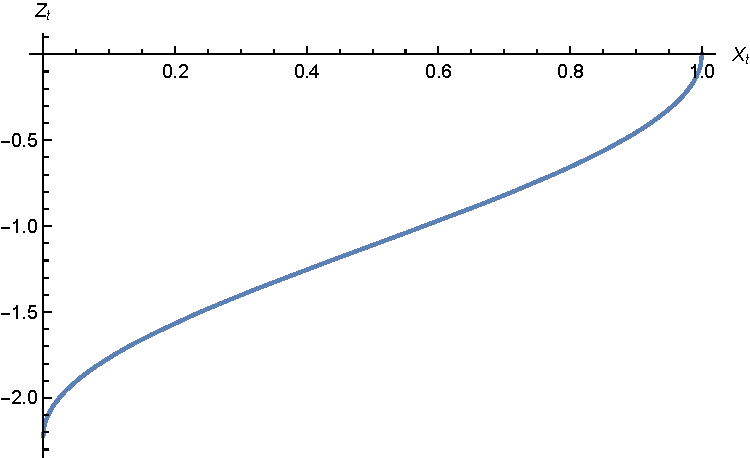
\includegraphics[width=0.8\textwidth]{../../Mathematica_Files/Range_Z.pdf}
%\end{figure}
%
%\end{columns}
%
%\end{frame}
%
%%%%%%%%%%%%%%%%%%%%%%%%%%%%%%%%%%%%%%%%%%%%%%%%%%%%
%
%\setbeamercolor{background canvas}{bg=white!20}
%\begin{frame}\frametitle{Estimation of $(\theta_0,\alpha,\epsilon)$: $\theta_0^*$ using LSM over different sets}
%
%Files: \textbf{MATLAB\_Files/Results/epsilon}: \textbf{theta\_0.eps} and \textbf{num\_over\_eps\_t0.eps} (plot\_epsilon.m, third cell).\\
%
%\begin{figure}[ht!]
%\centering
%\includegraphics[width=0.3\textwidth]{../../MATLAB_Files/Results/epsilon/theta_0.eps}\quad\quad
%\includegraphics[width=0.3\textwidth]{../../MATLAB_Files/Results/epsilon/num_over_eps_t0.eps}
%\end{figure}
%
%On the right, the number of samples as a function of $\gamma$. This samples satisfies that $p_i\in[\gamma,1-\gamma]$. On the left, the LSM over the samples that satisfies the $\gamma$ condition.
%
%\end{frame}
%
%%%%%%%%%%%%%%%%%%%%%%%%%%%%%%%%%%%%%%%%%%%%%%%%%%%%
%
%\setbeamercolor{background canvas}{bg=white!20}
%\begin{frame}\frametitle{Estimation of $(\theta_0,\alpha,\epsilon)$: $\epsilon$ using LSM over different sets}
%
%Files: \textbf{MATLAB\_Files/Results/epsilon}: \textbf{LSM.eps} and \textbf{num\_over\_eps.eps} (plot\_epsilon.m, second cell).\\
%
%\begin{figure}[ht!]
%\centering
%\includegraphics[width=0.3\textwidth]{../../MATLAB_Files/Results/epsilon/LSM.eps}\quad\quad
%\includegraphics[width=0.3\textwidth]{../../MATLAB_Files/Results/epsilon/num_over_eps.eps}
%\end{figure}
%
%On the right, the number of samples as a function of $\epsilon$. This samples satisfies that $p_i^\epsilon\in\{\epsilon,1-\epsilon\}$. On the left, the LSM for $\epsilon$,over the samples that satisfies the $\epsilon$ condition.
%
%\end{frame}
%
%%%%%%%%%%%%%%%%%%%%%%%%%%%%%%%%%%%%%%%%%%%%%%%%%%%%
%
%\setbeamercolor{background canvas}{bg=white!10}
%\begin{frame}\frametitle{$\delta$ over $\eta$:}
%
%Files: \textbf{MATLAB\_Files/Results/delta}: \textbf{eta\_min\_ini.eps} and \textbf{eta\_min\_opt.eps} (initiasl\_time.m, second cell).\\
%
%\begin{figure}[ht!]
%\centering
%\includegraphics[width=0.3\textwidth]{../../MATLAB_Files/Results/delta/eta_min_ini.eps}\quad\quad
%\includegraphics[width=0.3\textwidth]{../../MATLAB_Files/Results/delta/eta_min_opt.eps}
%\end{figure}
%We use the initial transitions that satisfies $|\Delta V|<\eta$. On the left, we use the initial $(\theta_0,\alpha)$ ($\alpha\theta_0=0.098$) and we get $\delta=\SI{220}{\min}$. On the right, we use the optimal ones. As the optimal product $\alpha\theta_0$ ($\alpha\theta_0=0.083$) is smaller than the initial one, we need either a larger $\delta$ to match the variance of the initial error, or to remove some data.
%\end{frame}
%
%%%%%%%%%%%%%%%%%%%%%%%%%%%%%%%%%%%%%%%%%%%%%%%%%%%%
%
%\setbeamercolor{background canvas}{bg=white!10}
%\begin{frame}\frametitle{Probability bands for model with delay:}
%Files: \textbf{MATLAB\_Files/Results/bands\_testing\_days/model\_1} (path\_simulator\_OPT\_model\_1.m).
%
%\begin{figure}[ht!]
%\centering
%\includegraphics[width=0.3\textwidth]{../../MATLAB_Files/Results/bands_testing_days/model_1/1.eps}
%\includegraphics[width=0.3\textwidth]{../../MATLAB_Files/Results/bands_testing_days/model_1/2.eps}
%\includegraphics[width=0.3\textwidth]{../../MATLAB_Files/Results/bands_testing_days/model_1/3.eps}
%\end{figure}
%
%We used the optimal parameters of the error SDE. We have results for the 128 testing days.
%
%\end{frame}
%
%%%%%%%%%%%%%%%%%%%%%%%%%%%%%%%%%%%%%%%%%%%%%%%%%%%%
%
%\setbeamercolor{background canvas}{bg=white!10}
%\begin{frame}\frametitle{Probability bands for Lamperti:}
%Files: \textbf{MATLAB\_Files/Results/bands\_testing\_days/lamperti\_optimal} (path\_simulator\_Lamperti.m).
%
%\begin{figure}[ht!]
%\centering
%\includegraphics[width=0.3\textwidth]{../../MATLAB_Files/Results/bands_testing_days/lamperti_optimal/1.eps}
%\includegraphics[width=0.3\textwidth]{../../MATLAB_Files/Results/bands_testing_days/lamperti_optimal/2.eps}
%\includegraphics[width=0.3\textwidth]{../../MATLAB_Files/Results/bands_testing_days/lamperti_optimal/3.eps}
%\end{figure}
%
%We used the Lamperti optimal parameters to simulate the Lamperti SDE. We have results for the 128 testing days.
%
%\end{frame}
%
%%%%%%%%%%%%%%%%%%%%%%%%%%%%%%%%%%%%%%%%%%%%%%%%%%%%
%
%\setbeamercolor{background canvas}{bg=white!10}
%\begin{frame}\frametitle{Paths for Lamperti:}
%Files: \textbf{MATLAB\_Files/Results/paths\_testing\_days/lamperti\_optimal} (path\_simulator\_Lamperti.m).
%
%\begin{figure}[ht!]
%\centering
%\includegraphics[width=0.3\textwidth]{../../MATLAB_Files/Results/paths_testing_days/lamperti_optimal/1.eps}
%\includegraphics[width=0.3\textwidth]{../../MATLAB_Files/Results/paths_testing_days/lamperti_optimal/2.eps}
%\includegraphics[width=0.3\textwidth]{../../MATLAB_Files/Results/paths_testing_days/lamperti_optimal/3.eps}
%\end{figure}
%
%We used the Lamperti optimal parameters to simulate the Lamperti SDE. We have results for the 128 testing days.
%
%\end{frame}
%
%%%%%%%%%%%%%%%%%%%%%%%%%%%%%%%%%%%%%%%%%%%%%%%%%%%%
%
%\setbeamercolor{background canvas}{bg=white!10}
%\begin{frame}\frametitle{Optimal $\delta$:}
%
%\begin{columns}
%
%\column{.5\textwidth}
%Files: \textbf{MATLAB\_Files/Results/delta} (initial\_time.m).\\
%\quad\\
%We can see that the optimal $\delta$ is highly dependent on the product $\theta_0\alpha$. This is because, that product represents the diffusion, which is predominant in the estimation of $\delta$.
%
%\column{.5\textwidth}
%\begin{figure}[ht!]
%\centering
%\includegraphics[width=1\textwidth]{../../MATLAB_Files/Results/delta/contour_delta.eps}
%\end{figure}
%
%\end{columns}
%
%\end{frame}
%
%%%%%%%%%%%%%%%%%%%%%%%%%%%%%%%%%%%%%%%%%%%%%%%%%%%%
%
%\setbeamercolor{background canvas}{bg=white!10}
%\begin{frame}\frametitle{Error transitions histograms:}
%Files: \textbf{MATLAB\_Files/Results/histograms/classic} (histogram\_classic\_SDE.m).\\
%\begin{figure}[ht!]
%\centering
%\includegraphics[width=0.4\textwidth]{../../MATLAB_Files/Results/histograms/classic/Optimal.eps}
%\includegraphics[width=0.4\textwidth]{../../MATLAB_Files/Results/histograms/classic/Lamperti_Optimal.eps}
%\end{figure}
%
%We can see two histograms for the error transitions. On the left, using $(\theta_0^E,\alpha^E)$, while on the right, using $(\theta_0^L,\alpha^L)$.
%
%\end{frame}
%
%%%%%%%%%%%%%%%%%%%%%%%%%%%%%%%%%%%%%%%%%%%%%%%%%%%%
%
%\setbeamercolor{background canvas}{bg=white!10}
%\begin{frame}\frametitle{Error transitions histograms:}
%Files: \textbf{MATLAB\_Files/Results/histograms/lamperti} (histogram\_lamperti\_SDE.m).\\
%\begin{figure}[ht!]
%\centering
%\includegraphics[width=0.4\textwidth]{../../MATLAB_Files/Results/histograms/lamperti/Optimal.eps}
%\includegraphics[width=0.4\textwidth]{../../MATLAB_Files/Results/histograms/lamperti/Optimal_Lamperti.eps}
%\end{figure}
%
%We can see two histograms for the error transitions. On the left, using $(\theta_0^E,\alpha^E)$, while on the right, using $(\theta_0^L,\alpha^L)$.
%
%\end{frame}
%
%%%%%%%%%%%%%%%%%%%%%%%%%%%%%%%%%%%%%%%%%%%%%%%%%%%%

\setbeamercolor{background canvas}{bg=white!10}
\begin{frame}\frametitle{Autocorrelation Function for the error observations $\{v_{j,i}\}_{j=1,i=1}^{M,N}$:}

\begin{figure}[ht!]
\centering
\includegraphics[width=0.4\textwidth]{../../MATLAB_Files/Results/Autocorrelation/observations.eps}
\end{figure}
We connect all the paths into a single and long path. Then, we compute the autocorrelation with lags from 0 to 200.

\end{frame}

\setbeamercolor{background canvas}{bg=white!10}
\begin{frame}\frametitle{Autocorrelation Function for the error transitions $\{\Delta v_{j,i}\}_{j=1,i=0}^{M,N}$:}

\begin{figure}[ht!]
\centering
\includegraphics[width=0.4\textwidth]{../../MATLAB_Files/Results/Autocorrelation/transitions.eps}
\end{figure}
We connect all the transitions. Then, we compute the autocorrelation with lags from 0 to 200.


\end{frame}

%%%%%%%%%%%%%%%%%%%%%%%%%%%%%%%%%%%

\setbeamercolor{background canvas}{bg=white!10}
\begin{frame}\frametitle{Cross-correlation Function for the error observations $\{v_{j,i}\}_{j=1,i=1}^{M,N}$:}

\begin{figure}[ht!]
\centering
\includegraphics[width=0.4\textwidth]{../../MATLAB_Files/Results/cross_correlation/obs_alldata.eps}
\end{figure}
We compute the cross-correlation between consecutive days. From the 147 days, we see the cross-correlation between 1-2, 2-3, $\dots$, and 146-147, with lags from -150 to 150.
\end{frame}

%%%%%%%%%%%%%%%%%%%%%%%%%%%%%%%%%%%

\setbeamercolor{background canvas}{bg=white!10}
\begin{frame}\frametitle{Cross-correlation Function for the error observations $\{v_{j,i}\}_{j=1,i=1}^{M,N}$:}

\begin{figure}[ht!]
\centering
\includegraphics[width=0.4\textwidth]{../../MATLAB_Files/Results/cross_correlation/obs_training.eps}
\end{figure}
We compute the cross-correlation between consecutive days. In this case using the training data, which does not have consecutive days.

\end{frame}

%%%%%%%%%%%%%%%%%%%%%%%%%%%%%%%%%%%

\setbeamercolor{background canvas}{bg=white!10}
\begin{frame}\frametitle{Cross-correlation Function for Lamperti observations $\{z_{j,i}\}_{j=1,i=1}^{M,N}$:}

\begin{figure}[ht!]
\centering
\includegraphics[width=0.4\textwidth]{../../MATLAB_Files/Results/cross_correlation/obs_alldata_L.eps}
\end{figure}
We compute the cross-correlation between consecutive days. From the 147 days, we see the cross-correlation between 1-2, 2-3, $\dots$, and 146-147, with lags from -150 to 150.
\end{frame}

%%%%%%%%%%%%%%%%%%%%%%%%%%%%%%%%%%%

\setbeamercolor{background canvas}{bg=white!10}
\begin{frame}\frametitle{Cross-correlation Function for Lamperti observations $\{z_{j,i}\}_{j=1,i=1}^{M,N}$:}

\begin{figure}[ht!]
\centering
\includegraphics[width=0.4\textwidth]{../../MATLAB_Files/Results/cross_correlation/obs_training_L.eps}
\end{figure}
We compute the cross-correlation between consecutive days. In this case using the training data, which does not have consecutive days.

\end{frame}

%%%%%%%%%%%%%%%%%%%%%%%%%%%%%%%%%%%

\end{document}